\chapter{Стационарное действие и уравнение Эйлера--Лагранжа}

\lectureoverview{Привычное название \emph{принцип наименьшего действия} скрывает существенный момент: физическая траектория делает действие стационарным, но не обязана его минимизировать. Мы выведем это утверждение из обычного равновесия, распространим его с точек на целые функции, получим уравнение Эйлера--Лагранжа, дискретизуя путь, и восстановим уравнения Ньютона. Затем вращающиеся и полярные координаты покажут, почему лагранжева формулировка — это не просто смена обозначений.}

\section{Стационарно, но не обязательно минимально}

Слово \emph{наименьшего} — ненадежная часть традиционного названия. Классическая траектория не всегда делает действие минимумом. Вместо этого она может давать максимум или седло в пространстве возможных траекторий. Правильный принцип состоит в том, что действие \emph{стационарно}: его изменение первого порядка обращается в нуль.

Начнем с более простого вопроса о равновесии. Частица, остающаяся в покое, не имеет ускорения, поэтому равнодействующая сил должна обращаться в нуль. Для силы, получаемой из одномерного потенциала, \begin{equation}
  F(x)=-\frac{dV}{dx},
  \label{eq:force-from-v}
\end{equation} условие равновесия имеет вид \begin{equation}
  \frac{dV}{dx}=0.
  \label{eq:stationary-v-one}
\end{equation}

\begin{figure}[htbp] \centering
  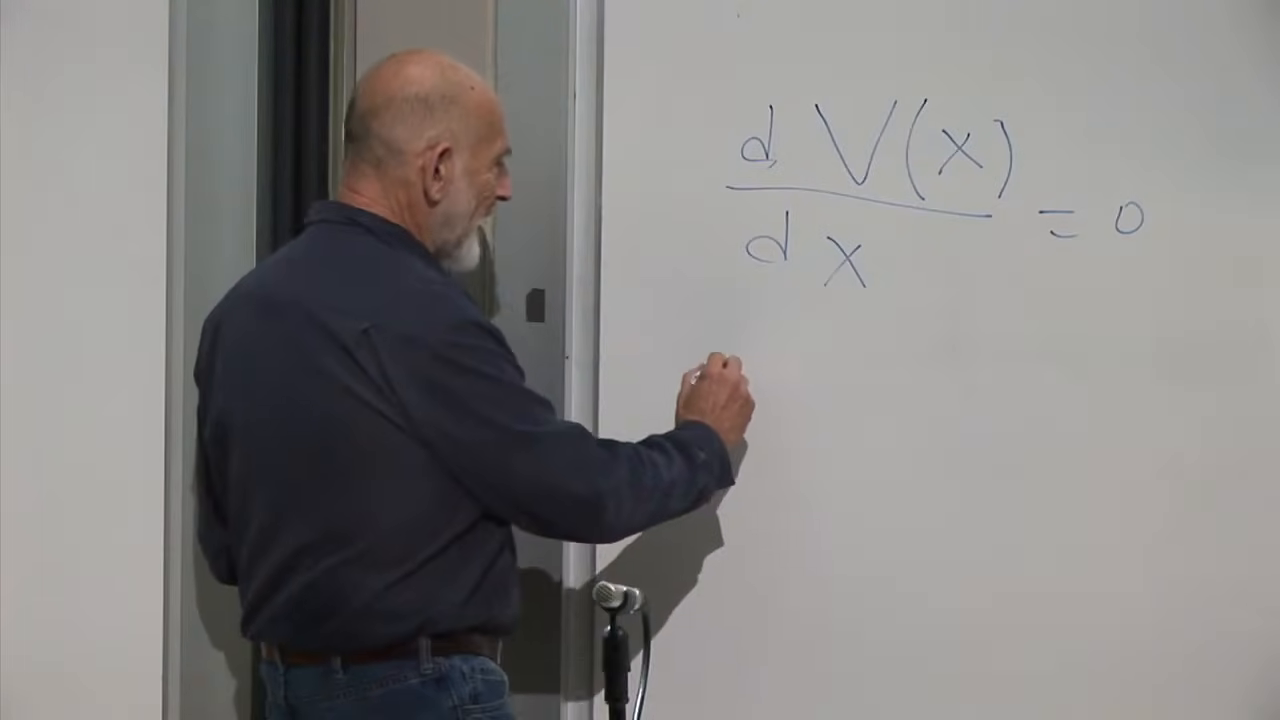
\includegraphics[width=0.74\textwidth]{lecture_03_figure_02.png} \caption{Одномерное условие равновесия: сила обращается в нуль там, где потенциал стационарен.} \lectureframe{00:02:51} \end{figure}

Теперь сместим частицу на малую величину \(\delta x\). В первом порядке \begin{equation}
  \delta V
  =V(x+\delta x)-V(x)
  =\frac{dV}{dx}\,\delta x+O(\delta x^2).
  \label{eq:first-variation-one}
\end{equation} В равновесии линейный член равен нулю при любом знаке \(\delta x\): \begin{equation}
  \delta V=0
  \qquad\hbox{to first order.}
  \label{eq:delta-v-zero-one}
\end{equation} Это не означает, что \(V\) точно не меняется после конечного смещения. Это означает, что главное изменение имеет квадратичный или более высокий порядок. И минимум, и максимум удовлетворяют этому условию.

\begin{figure}[htbp] \centering
  \begin{tikzpicture}[scale=0.95,>=Latex]
    \draw[->] (-0.2,0) -- (3.35,0) node[right] {$x$};
    \draw[->] (0,-0.2) -- (0,2.25) node[above] {$V$};
    \draw[blue!65!black,thick,smooth]
      plot coordinates {(0.2,1.85) (0.75,0.85) (1.55,0.35)
                        (2.35,0.85) (3.0,1.85)};
    \fill[red!65!black] (1.55,0.35) circle (2pt);
    \node at (1.55,-0.34) {minimum};
    \begin{scope}[xshift=4.25cm]
      \draw[->] (-0.2,0) -- (3.35,0) node[right] {$x$};
      \draw[->] (0,-0.2) -- (0,2.25) node[above] {$V$};
      \draw[blue!65!black,thick,smooth]
        plot coordinates {(0.2,0.35) (0.75,1.25) (1.55,1.85)
                          (2.35,1.25) (3.0,0.35)};
      \fill[red!65!black] (1.55,1.85) circle (2pt);
      \node at (1.55,-0.34) {maximum};
    \end{scope}
  \end{tikzpicture} \caption{Стационарность определяет первую производную, но не то, является ли точка минимумом или максимумом.} \label{fig:min-max-stationary} \end{figure}

Для многих координат \(q_i\) первая вариация равна \begin{equation}
  \delta V
  =\sum_i\frac{\partial V}{\partial q_i}\,\delta q_i.
  \label{eq:first-variation-many}
\end{equation} Если она должна обращаться в нуль при любых независимых бесконечно малых смещениях \(\delta q_i\), то каждый коэффициент обращается в нуль: \begin{equation}
  \frac{\partial V}{\partial q_i}=0
  \qquad\hbox{for every }i.
  \label{eq:stationary-v-many}
\end{equation}

Двумерный потенциал лучше представлять себе не как американские горки, а как холмистую местность. Стационарная точка может быть дном долины, вершиной холма или седлом. В седле движение в одном направлении сначала идет вверх, тогда как в другом сначала идет вниз. Поэтому восстанавливающее поведение может быть устойчивым в одном направлении и неустойчивым в другом, хотя все первые производные в самой точке обращаются в нуль.

\begin{figure}[htbp] \centering
  \includegraphics[width=0.76\textwidth]{lecture_03_figure_06.png} \caption{Седло стационарно в первом порядке по любому направлению, хотя соседние смещения вдоль одной оси ведут вверх, а вдоль другой — вниз.} \lectureframe{00:08:20} \end{figure}

В пространстве со многими координатами седловые точки более типичны, чем чистые максимумы или минимумы. Поэтому ключевым словом остается \emph{стационарное}. Условие \begin{equation}
  \delta V=0
  \label{eq:equilibrium-variation}
\end{equation} выражает равновесие, не предрешая поведения второго порядка.

\section{От точек к функциям}

Механика занимается целыми движениями, а не изолированными точками равновесия. Траектория — это функция, такая как \(x(t)\), или совокупность \((x(t),y(t),z(t))\). Математическая задача сделать некоторую величину стационарной, варьируя целую функцию, составляет \emph{вариационное исчисление}. Прежде чем применять его к движению, рассмотрим три более простых примера.

\subsection{Кратчайшие кривые и геодезические}

Зафиксируем две точки на плоскости и представим кривую между ними как \(y(x)\). На коротком участке \begin{equation}
  ds=\sqrt{dx^2+dy^2}
  =dx\sqrt{1+\left(\frac{dy}{dx}\right)^2},
  \label{eq:line-element}
\end{equation} где последняя форма предполагает \(dx>0\). Полная длина есть функцион \begin{equation}
  S[y]=\int_{x_0}^{x_1}
  \sqrt{1+y'(x)^2}\,dx.
  \label{eq:arc-length-functional}
\end{equation} Квадратные скобки подчеркивают, что \(S\) принимает в качестве аргумента целую функцию. Прямая линия выделяется условием \begin{equation}
  \delta S=0
  \label{eq:stationary-length}
\end{equation} при малых изменениях кривой, оставляющих оба конца фиксированными.

\begin{figure}[htbp] \centering
  \includegraphics[width=0.78\textwidth]{lecture_03_figure_07.png} \caption{Пробная кривая между двумя фиксированными концами. Ее длина есть сумма бесконечно малых гипотенуз \(ds\).} \lectureframe{00:13:36} \end{figure}

Тот же вопрос можно задать на искривленной поверхности. Натягивание нити между двумя колышками дает физическую картину кратчайшего пути, ограниченного этой поверхностью. Такая кривая со стационарной длиной — \emph{геодезическая}. На плоскости это прямая линия; на сфере или холмистой поверхности — вообще говоря, нет.

\subsection{Принцип Ферма}

Луч света в среде, где скорость зависит от положения \(c(x,y)\), не обязан следовать по кратчайшему пространственному пути. Время, необходимое для малого участка, равно расстоянию, деленному на локальную скорость, так что \begin{equation}
  T[y]
  =\int_{x_0}^{x_1}
  \frac{\sqrt{1+y'(x)^2}}{c(x,y)}\,dx.
  \label{eq:fermat-functional}
\end{equation} Принцип Ферма требует \begin{equation}
  \delta T=0.
  \label{eq:fermat-stationary}
\end{equation} Если скорость \(c\) постоянна, это сводится к задаче о кратчайшем расстоянии. Однако в среде с переменным показателем преломления быстрейший путь уравновешивает длину пути и локальную скорость распространения.

\begin{figure}[htbp] \centering
  \includegraphics[width=0.80\textwidth]{lecture_03_figure_08.png} \caption{Функционал наименьшего времени для луча в среде, где локальная скорость света зависит от положения.} \lectureframe{00:22:50} \end{figure}

Злободневная шутка отсылает к тогдашнему недавнему заявлению, что в Италии нейтрино двигались необычно быстро. Физический довод сразу возвращается к надежному примеру: обычный свет меняет скорость в веществе в соответствии с показателем преломления.

\subsection{Висящая цепь}

Цепь, закрепленная в двух точках, принимает форму цепной линии. Каждый малый участок вносит вклад в гравитационную потенциальную энергию, так что полная потенциальная энергия сама представляет собой интеграл по цепи. И снова концы фиксированы, неизвестная форма задается функцией, и интеграл должен быть стационарным.

\begin{figure}[htbp] \centering
  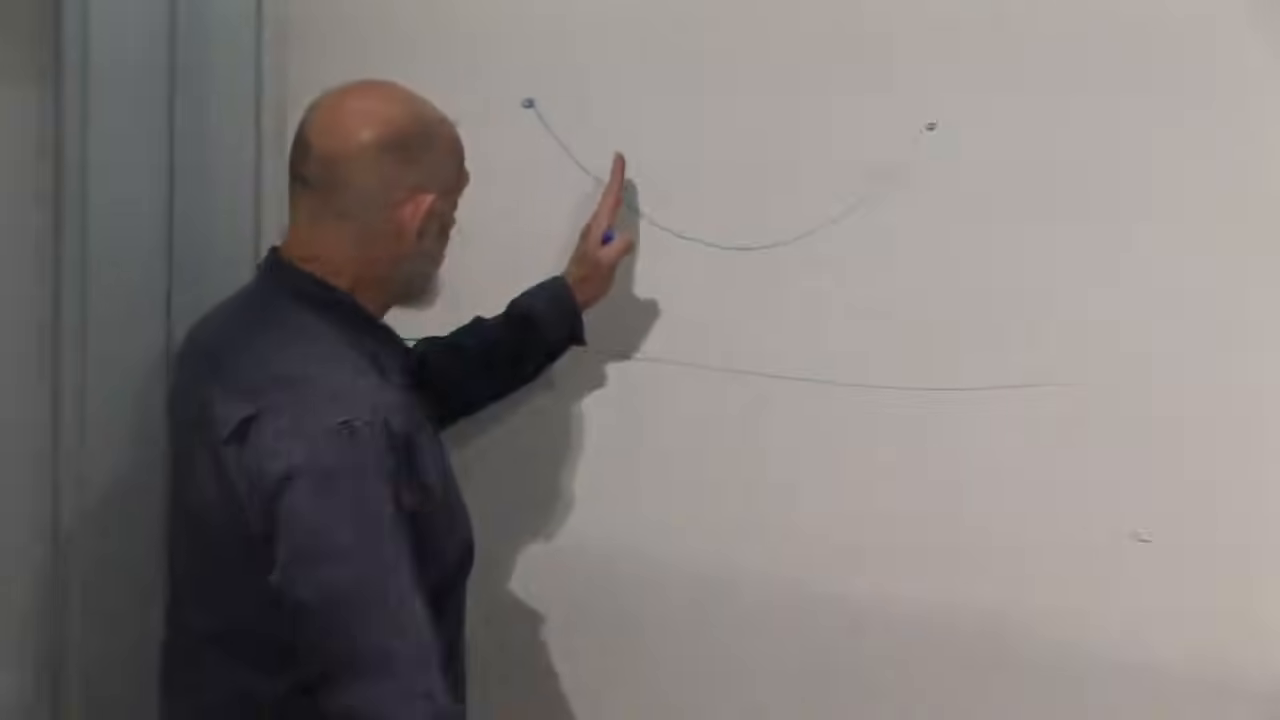
\includegraphics[width=0.76\textwidth]{lecture_03_figure_03.png} \caption{Висящая цепь между фиксированными опорами. Ее стационарная форма определяется полной гравитационной потенциальной энергией.} \lectureframe{00:30:41} \end{figure}

У этих примеров одна и та же структура: два фиксированных конца, функция между ними и интеграл, первая вариация которого обращается в нуль. Свести такое глобальное предписание к дифференциальному уравнению и значит решить вариационную задачу.

\section{Механика как краевая задача}

Траекторию часто изображают с горизонтальной осью времени, потому что \(t\) — независимая переменная. Тем не менее в физике существует устойчивая традиция изображать время направленным вверх. В сторону заметим, что в экспериментах люди располагали картинки от юности к старости в направлениях, связанных с их системами письма: читающие слева направо обычно размещали их слева направо, читающие справа налево — наоборот, а обученные вертикальному письму — по вертикали. Шутка заключает, что физики — это люди, которые настаивают на том, что время течет вверх. Здесь мы будем использовать обычную горизонтальную ось \(t\), потому что тогда \(x(t)\) естественно читается как график.

В формулировке с начальными условиями данные при \(t_0\) имеют вид \begin{equation}
  x(t_0)=x_0,
  \qquad
  \dot x(t_0)=v_0.
  \label{eq:initial-value-data}
\end{equation} Уравнение Ньютона затем определяет дальнейшую траекторию. Вариационная формулировка ставит другую задачу: задать два концевых события, \begin{equation}
  x(t_0)=x_0,
  \qquad
  x(t_1)=x_1,
  \label{eq:boundary-value-data}
\end{equation} и определить физический путь между ними. Начальная скорость больше не задается; она становится частью решения.

\begin{figure}[htbp] \centering
  \includegraphics[width=0.76\textwidth]{lecture_03_figure_09.png} \caption{Механическая траектория \(x(t)\). Можно задать положение и наклон на одном конце либо положения в двух конечных моментах времени.} \lectureframe{00:27:41} \end{figure}

Величина, которую нужно сделать стационарной, — это \emph{действие}, \begin{equation}
  A[x]=\int_{t_0}^{t_1}L(x,\dot x,t)\,dt.
  \label{eq:action-one}
\end{equation} Подынтегральная функция \(L\) — это \emph{функция Лагранжа}. Она может зависеть от положения, скорости и явно от времени. Принцип действия имеет вид \begin{equation}
  \delta A=0
  \label{eq:stationary-action}
\end{equation} для всех малых вариаций пути, при которых \begin{equation}
  \delta x(t_0)=\delta x(t_1)=0.
  \label{eq:fixed-endpoint-variations}
\end{equation} Условие на концах существенно: мы сравниваем соседние пути, соединяющие одни и те же два события.

\section{Дискретный вывод уравнения Эйлера--Лагранжа}

Действие является функционалом бесконечно многих значений траектории. Чтобы сделать его вариацию наглядной, разобьем интервал времени на шаги длины \(\epsilon\), \begin{equation}
  t_n=t_0+n\epsilon,
  \qquad
  x_n=x(t_n),
  \label{eq:discrete-times}
\end{equation} и аппроксимируем скорость на \(n\)-м интервале выражением \begin{equation}
  v_n=\frac{x_{n+1}-x_n}{\epsilon}.
  \label{eq:discrete-velocity}
\end{equation} Интеграл превращается в обычную сумму \begin{equation}
  A_\epsilon
  =\sum_{n=0}^{N-1}
  \epsilon L\left(x_n,\frac{x_{n+1}-x_n}{\epsilon}\right).
  \label{eq:discrete-action}
\end{equation} Мы используем \(n\) как индекс временного слоя, чтобы \(i\) позже можно было использовать для пространственных координат и частиц.

\begin{figure}[htbp] \centering
  \includegraphics[width=0.82\textwidth]{lecture_03_figure_10.png} \caption{Траектория, замененная цепочкой временных слоев. Варьирование одной внутренней ординаты изменяет только два соседних с ней отрезка.} \lectureframe{00:38:30} \end{figure}

Проварьируем одну внутреннюю точку \(x_n\), удерживая все остальные \(x_k\) фиксированными. Только два члена суммы зависят от \(x_n\): \begin{align}
  A_\epsilon\big|_{x_n}
  &=
  \epsilon L\left(x_n,\frac{x_{n+1}-x_n}{\epsilon}\right)
  \notag\\
  &\quad+
  \epsilon L\left(x_{n-1},
                  \frac{x_n-x_{n-1}}{\epsilon}\right).
  \label{eq:two-neighbor-terms}
\end{align} Дифференцируя, получаем \begin{align}
  0=\frac{\partial A_\epsilon}{\partial x_n}
  &=
  \epsilon\frac{\partial L_n}{\partial x_n}
  -\frac{\partial L_n}{\partial v_n}
  +\frac{\partial L_{n-1}}{\partial v_{n-1}}.
  \label{eq:discrete-el-variation}
\end{align} Противоположные знаки имеют простое геометрическое происхождение. Увеличение \(x_n\) увеличивает наклон предшествующего ему интервала и уменьшает наклон следующего за ним интервала.

\begin{figure}[htbp] \centering
  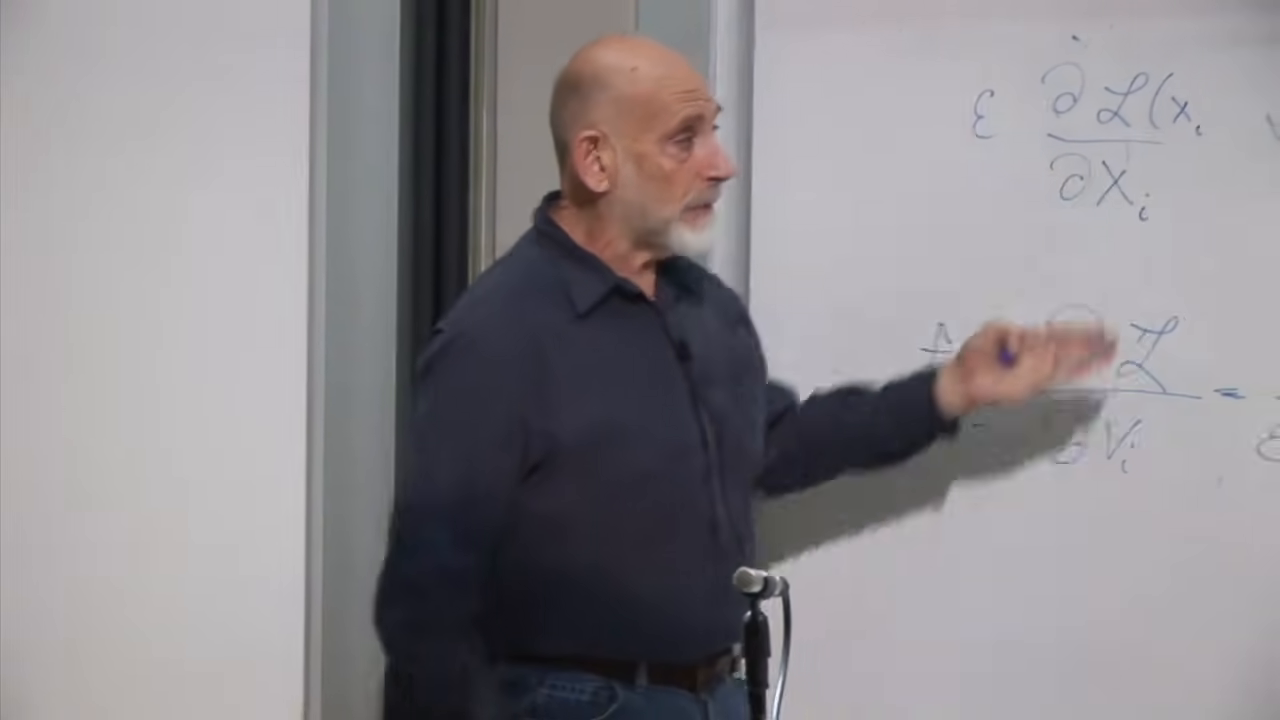
\includegraphics[width=0.74\textwidth]{lecture_03_figure_04.png} \caption{Непосредственная производная по координате и два соседних вклада от производных по скорости в дискретной вариации.} \lectureframe{00:45:26} \end{figure}

Перегруппируем уравнение~\eqref{eq:discrete-el-variation}:
\begin{equation}
  \frac{1}{\epsilon}
  \left(
    \frac{\partial L_n}{\partial v_n}
    -\frac{\partial L_{n-1}}{\partial v_{n-1}}
  \right)
  =
  \frac{\partial L_n}{\partial x_n}.
  \label{eq:discrete-el}
\end{equation}
Левая часть — разностное отношение по соседним точкам. При \(\epsilon\to0\) ломаная превращается в гладкую траекторию, а это отношение становится производной по времени:
\begin{equation}
  \boxed{
  \frac{d}{dt}\left(\frac{\partial L}{\partial\dot x}\right)
  =
  \frac{\partial L}{\partial x}}
  .
  \label{eq:euler-lagrange-one}
\end{equation}
Это уравнение Эйлера--Лагранжа.

\begin{figure}[htbp]
  \centering
  \includegraphics[width=0.78\textwidth]{lecture_03_figure_11.png}
  \caption{Полное уравнение Эйлера--Лагранжа, полученное из условия стационарности на каждом внутреннем временном срезе.}
  \lectureframe{00:49:25}
\end{figure}

Как только задан \(L\), уравнение~\eqref{eq:euler-lagrange-one} работает как вычислительный механизм: продифференцируйте данную функцию, и он выдаст дифференциальное уравнение для траектории.

\begin{classroomqa}
  \audiencequestion{Верно ли результат Эйлера--Лагранжа для любой функции от \(x\) и \(\dot x\)?\lecturetimestamp{00:49:37--00:50:24}}
  \lecturerresponse{Да, при условии той регулярности, которая нужна для существования производных. Пример с длиной дуги после переобозначения имеет в точности ту же форму: его независимая переменная \(x\) играет ту роль, которую здесь играет \(t\), а его неизвестная функция \(y(x)\) — ту роль, которую здесь играет \(x(t)\). Его уравнение Эйлера--Лагранжа имеет решения в виде прямых линий.}
\end{classroomqa}

\section{Уравнения Ньютона из лагранжиана}

Для частицы на прямой в потенциале \(V(x)\) возьмём
\begin{equation}
  L(x,\dot x)=T-V
  =\frac12m\dot x^2-V(x).
  \label{eq:lagrangian-tv-one}
\end{equation}
Знак минус может показаться странным, потому что полная энергия равна \(T+V\). Но лагранжиан — не энергия. Критерий состоит в том, выдаёт ли механизм Эйлера--Лагранжа правильное движение. Устраивать шуточное голосование по поводу знака не будем: ответ нужно проверять, а не выбирать голосованием.

Сначала,
\begin{equation}
  \frac{\partial L}{\partial\dot x}=m\dot x.
  \label{eq:conjugate-momentum-one}
\end{equation}
Это импульс. В более общем случае импульс, сопряжённый любой координате \(q\), определяется как
\begin{equation}
  p_q=\frac{\partial L}{\partial\dot q}.
  \label{eq:conjugate-momentum-general}
\end{equation}
Взяв производную по времени от уравнения~\eqref{eq:conjugate-momentum-one}, получаем \(m\ddot x\), тогда как
\begin{equation}
  \frac{\partial L}{\partial x}
  =-\frac{dV}{dx}.
  \label{eq:lagrangian-position-derivative}
\end{equation}
Следовательно, уравнение Эйлера--Лагранжа имеет вид
\begin{equation}
  m\ddot x=-\frac{dV}{dx}=F(x),
  \label{eq:newton-from-action}
\end{equation}
что и есть второй закон Ньютона.

\begin{figure}[htbp]
  \centering
  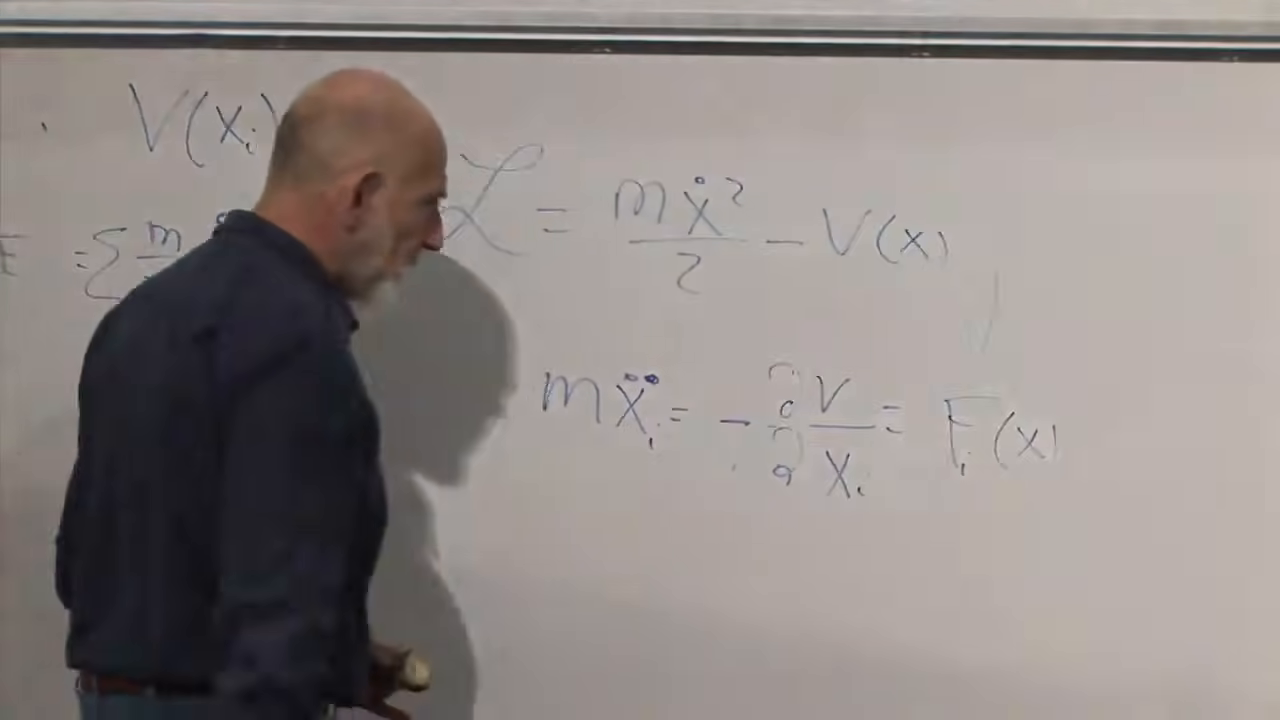
\includegraphics[width=0.80\textwidth]{lecture_03_figure_05.png}
  \caption{Кинетическая энергия, потенциальная энергия, \(L=T-V\) и восстановленная покомпонентная форма уравнения Ньютона на одной доске.}
  \lectureframe{00:57:52}
\end{figure}

Для многих координат \(q_i\),
\begin{equation}
  L(\mathbf q,\dot{\mathbf q})
  =\sum_i\frac12m_i\dot q_i^{\,2}-V(q_1,q_2,\ldots),
  \label{eq:lagrangian-tv-many}
\end{equation}
и для каждой координаты имеется своё уравнение:
\begin{equation}
  \frac{d}{dt}\left(\frac{\partial L}{\partial\dot q_i}\right)
  =\frac{\partial L}{\partial q_i}
  \quad\Longrightarrow\quad
  m_i\ddot q_i=-\frac{\partial V}{\partial q_i}=F_i.
  \label{eq:euler-lagrange-many}
\end{equation}
Траектория по-прежнему остаётся одной кривой, теперь в многомерном конфигурационном пространстве.

\begin{classroomqa}
  \audiencequestion{Неужели мы всего лишь пошли в обратную сторону от закона Ньютона и сконструировали функционал, воспроизводящий ответ?\lecturetimestamp{00:58:07--01:00:04}}
  \lecturerresponse{Это не самая продуктивная точка зрения. Лагранжиан — компактное задание физической системы: одна функция всех координат и скоростей заключает в себе все её уравнения движения. В новых теориях физики обычно предлагают действие и выводят уравнения, а не угадывают каждое уравнение по отдельности.}
\end{classroomqa}

Такая компактная запись — одно из преимуществ. Свобода выбора координат — другое. Утверждение о том, что прямая — кратчайшая линия, не зависит от того, описывается ли плоскость декартовыми, полярными или криволинейными координатами. Точно так же стационарность действия не зависит от выбора координат, хотя формула для \(L\) и получающиеся покомпонентные уравнения меняются.

\section{Свободная частица, наблюдаемая с карусели}

Пусть \((x,y)\) — инерциальные декартовы координаты, а \((X,Y)\) — координаты, равномерно вращающиеся с угловой скоростью \(\omega\). При выбранной здесь ориентации,
\begin{align}
  x&=X\cos\omega t+Y\sin\omega t,
  \notag\\
  y&=-X\sin\omega t+Y\cos\omega t.
  \label{eq:rotating-coordinate-map}
\end{align}
Угол между системами координат равен \(\omega t\).

\begin{figure}[htbp]
  \centering
  \includegraphics[width=0.76\textwidth]{lecture_03_figure_12.png}
  \caption{Инерциальные и равномерно вращающиеся декартовы оси. Одной и той же точке сопоставляются зависящие от времени вращающиеся координаты.}
  \lectureframe{01:06:05}
\end{figure}

Для свободной частицы лагранжиан в инерциальной системе имеет вид
\begin{equation}
  L_{\mathrm{in}}
  =\frac{m}{2}\left(\dot x^2+\dot y^2\right).
  \label{eq:free-inertial-lagrangian}
\end{equation}
Продифференцируем уравнение~\eqref{eq:rotating-coordinate-map} и воспользуемся \(\sin^2\omega t+\cos^2\omega t=1\). Тригонометрические члены объединяются, давая
\begin{align}
  \dot x^2+\dot y^2
  &=
  \dot X^2+\dot Y^2\\
  &\quad+\omega^2(X^2+Y^2)\\
  &\quad+2\omega(Y\dot X-X\dot Y).
  \label{eq:rotating-speed}
\end{align}
Следовательно,
\begin{align}
  L_{\mathrm{rot}}
  &=
  \frac{m}{2}(\dot X^2+\dot Y^2)\\
  &\quad+\frac{m\omega^2}{2}(X^2+Y^2)\\
  &\quad+m\omega(Y\dot X-X\dot Y).
  \label{eq:rotating-lagrangian}
\end{align}

\begin{figure}[htbp]
  \centering
  \includegraphics[width=0.84\textwidth]{lecture_03_figure_13.png}
  \caption{Преобразованный лагранжиан свободной частицы: обычная кинетическая энергия, квадратичный центробежный член и член, линейный по скорости.}
  \lectureframe{01:12:16}
\end{figure}

Квадратичный по координатам член имеет вид \(-V_{\mathrm{fict}}\), где
\begin{equation}
  V_{\mathrm{fict}}
  =-\frac{m\omega^2}{2}(X^2+Y^2).
  \label{eq:centrifugal-potential}
\end{equation}
Он убывает при движении наружу, поэтому создаёт центробежную силу \(m\omega^2(X,Y)\).

Последний член в уравнении~\eqref{eq:rotating-lagrangian} линейный и по координатам, и по скоростям. Применение уравнения Эйлера--Лагранжа даёт
\begin{align}
  m\ddot X&=m\omega^2X-2m\omega\dot Y,
  \notag\\
  m\ddot Y&=m\omega^2Y+2m\omega\dot X.
  \label{eq:rotating-equations}
\end{align}
Члены, пропорциональные \(\omega^2\), являются центробежными; пропорциональные скорости — кориолисовыми. В векторной форме в плоскости вращения,
\begin{equation}
  \mathbf F_{\mathrm{C}}
  =-2m\,\boldsymbol\omega\times\mathbf v_{\mathrm{rot}},
  \label{eq:coriolis-vector}
\end{equation}
причём при выборе противоположной ориентации знаки следует изменить.

\begin{figure}[htbp]
  \centering
  \includegraphics[width=0.84\textwidth]{lecture_03_figure_14.png}
  \caption{Уравнения во вращающейся системе, в которых члены, пропорциональные координатам, дают центробежное ускорение, а перекрёстные скоростные члены — кориолисово ускорение.}
  \lectureframe{01:20:20}
\end{figure}

Суть не в том, что алгебра исчезает. Суть в том, что одно преобразование координат, применённое к одной скалярной функции, порождает и обе связанные уравнения, и обе фиктивные силы.

\begin{classroomqa}
  \audiencequestion{Работает ли этот метод для произвольно криволинейных координат?\lecturetimestamp{01:22:01--01:22:17}}
  \lecturerresponse{Да. Новые координаты могут быть криволинейными и даже явно зависеть от времени, как вращающиеся координаты. Перепишите действие в новых переменных и примените то же правило Эйлера--Лагранжа.}
\end{classroomqa}

\section{Полярные координаты и циклический угол}

Для обычных полярных координат,
\begin{equation}
  x=r\cos\theta,
  \qquad
  y=r\sin\theta.
  \label{eq:polar-map}
\end{equation}
И \(r\), и \(\theta\) могут зависеть от времени. После дифференцирования и сложения квадратов получаем
\begin{equation}
  \dot x^2+\dot y^2
  =\dot r^2+r^2\dot\theta^2.
  \label{eq:polar-speed}
\end{equation}
Для центрального потенциала \(V(r)\),
\begin{equation}
  L
  =\frac{m}{2}\left(\dot r^2+r^2\dot\theta^2\right)-V(r).
  \label{eq:polar-lagrangian}
\end{equation}

\begin{figure}[htbp]
  \centering
  \includegraphics[width=0.80\textwidth]{lecture_03_figure_15.png}
  \caption{Полярная геометрия и разложение кинетической энергии на радиальное и угловое движение.}
  \lectureframe{01:23:30}
\end{figure}

Радиальное уравнение имеет вид
\begin{equation}
  m\ddot r
  =mr\dot\theta^2-\frac{dV}{dr}.
  \label{eq:radial-equation}
\end{equation}
Первый член — направленный наружу центробежный вклад, связанный с собственным угловым движением частицы.

Для угла,
\begin{equation}
  \frac{d}{dt}\left(\frac{\partial L}{\partial\dot\theta}\right)
  =\frac{\partial L}{\partial\theta}=0,
  \label{eq:theta-el}
\end{equation}
поскольку центральный потенциал не имеет явной зависимости от \(\theta\). Следовательно,
\begin{equation}
  \frac{d}{dt}\left(mr^2\dot\theta\right)=0,
  \qquad
  mr^2\dot\theta=\ell,
  \label{eq:angular-momentum}
\end{equation}
где \(\ell\) — сохраняющийся момент импульса.

\begin{figure}[htbp]
  \centering
  \includegraphics[width=0.82\textwidth]{lecture_03_figure_16.png}
  \caption{Угловое уравнение Эйлера--Лагранжа имеет нулевую правую часть, выявляя сохранение \(mr^2\dot\theta\).}
  \lectureframe{01:29:25}
\end{figure}

Угловое уравнение даёт
\begin{equation}
  \dot\theta=\frac{\ell}{mr^2}.
  \label{eq:theta-dot-angular-momentum}
\end{equation}
Подстановка в уравнение~\eqref{eq:radial-equation} оставляет одно уравнение для \(r\):
\begin{equation}
  m\ddot r
  =\frac{\ell^2}{mr^3}-\frac{dV}{dr}.
  \label{eq:effective-radial-equation}
\end{equation}

Координату, отсутствующую в \(L\), традиционно называют \emph{циклической}, даже если она не является углом. Если \(q\) циклическая, то
\begin{equation}
  \frac{\partial L}{\partial q}=0
  \quad\Longrightarrow\quad
  \frac{d}{dt}\left(\frac{\partial L}{\partial\dot q}\right)=0.
  \label{eq:cyclic-conservation}
\end{equation}
Её сопряжённый импульс сохраняется. Это первое указание на общую связь между симметрией и законом сохранения.

\section{Вопросы о смысле, энергии и области применимости}

Следующие вопросы показывают, где заключено более глубокое содержание этого формализма.

\begin{classroomqa}
  \audiencequestion{Есть ли независимое основание прийти к лагранжиану, кроме обнаружения того, что он даёт правильные классические уравнения?\lecturetimestamp{01:33:25--01:35:07}}
  \lecturerresponse{Исторически более чем столетнее развитие классической механики показало, что частицы, волны и электромагнитные поля могут быть представлены в этой форме. На классическом уровне этот накопленный успех является эмпирическим фактом о том, как организованы законы. Более глубокое объяснение приходит из квантовой механики и пока откладывается.}
\end{classroomqa}

\begin{classroomqa}
  \audiencequestion{В лагранжиане во вращающейся системе можно ли отнести линейный по скорости член к обычной кинетической или потенциальной энергии?\lecturetimestamp{01:35:08--01:36:23}}
  \lecturerresponse{Нет. Сохраняющаяся величина, связанная со сдвигом по времени, получается гамильтоновым построением, а не из попытки читать каждый член в \(L\) как кинетическую или потенциальную энергию. Для уравнения~\eqref{eq:rotating-lagrangian} линейный по скорости член сокращается в \(\sum_a\dot q_a\,\partial L/\partial\dot q_a-L\). Гамильтонов подход систематизирует это.}
\end{classroomqa}

Действительно, поскольку \(L_{\mathrm{rot}}\) не зависит явно от времени,
\begin{equation}
  \begin{aligned}
    H_{\mathrm{rot}}
    &=\dot X\frac{\partial L}{\partial\dot X}
     +\dot Y\frac{\partial L}{\partial\dot Y}-L\\
    &=\frac{m}{2}(\dot X^2+\dot Y^2)
     -\frac{m\omega^2}{2}(X^2+Y^2)
  \end{aligned}
  \label{eq:rotating-hamiltonian-preview}
\end{equation}
сохраняется. Это интеграл Якоби во вращающейся системе, а не то же самое численное значение энергии, которое приписывает инерциальный наблюдатель. Зависящие от времени преобразования координат не обязаны сохранять численную форму энергии.

\begin{classroomqa}
  \audiencequestion{Что, если искривлённая траектория вызвана гравитацией?\lecturetimestamp{01:36:30--01:37:10}}
  \lecturerresponse{Для ньютоновской гравитации просто используйте \(V(r)=-GMm/r\) в лагранжиане центральной силы. Искривлённое пространство-время относится к общей теории относительности и здесь не предполагается.}
\end{classroomqa}

\begin{classroomqa}
  \audiencequestion{Не являются ли центробежный потенциал и соответствующая ему энергия всего лишь фиктивными?\lecturetimestamp{01:37:13--01:40:14}}
  \lecturerresponse{Наблюдатель на вращающейся платформе измеряет эффективные силы и может последовательно использовать сохраняющуюся величину во вращающейся системе. Слово \emph{фиктивный} означает, что эти члены возникают из неинерциального описания, а не что их наблюдаемые эффекты воображаемы. Сама энергия не инвариантна при общем зависящем от времени преобразовании координат.}
\end{classroomqa}

\begin{classroomqa}
\audiencequestion{Куда направлена зависящая от скорости сила Кориолиса?\lecturetimestamp{01:40:22--01:42:36}}
\lecturerresponse{Она перпендикулярна скорости во вращающейся системе отсчёта; её величина пропорциональна скорости и угловой скорости системы отсчёта. В плоскости компоненты меняют местами \(\dot X\) и \(\dot Y\) с противоположными знаками, как в уравнении~\eqref{eq:rotating-equations}.}
\end{classroomqa}

\begin{figure}[htbp]
\centering
  \includegraphics[width=0.76\textwidth]{lecture_03_figure_17.png}
\caption{Перекрёстная структура скоростных компонент: сила Кориолиса перпендикулярна скорости во вращающейся системе отсчёта.}
\lectureframe{01:41:40}
\end{figure}

\begin{classroomqa}
\audiencequestion{Должен ли исходный лагранжиан быть записан в инерциальной системе отсчёта?\lecturetimestamp{01:42:37--01:44:00}}
\lecturerresponse{Для обычной свободной частицы ньютоновский закон в инерциальной системе отсчёта даёт простую исходную форму \(m(\dot x^2+\dot y^2)/2\). Когда этот физический закон известен, действие можно преобразовать к любым другим координатам. Не следует независимо предполагать ту же простую кинетическую формулу во вращающейся системе отсчёта.}
\end{classroomqa}

Такой же тип линейного по скорости члена возникает для заряженной частицы в магнитном поле:
\begin{equation}
  L_{\mathrm{em}}
  =\frac12m\mathbf v^2
   +q\mathbf A(\mathbf r,t)\cdot\mathbf v
   -q\phi(\mathbf r,t).
  \label{eq:electromagnetic-lagrangian}
\end{equation}
Для однородного магнитного поля, перпендикулярного плоскости, симметричная калибровка \(\mathbf A=\tfrac12\mathbf B\times\mathbf r\) даёт член, пропорциональный \(X\dot Y-Y\dot X\), с той же алгебраической структурой, что и кориолисов член.

\begin{figure}[htbp]
\centering
  \includegraphics[width=0.82\textwidth]{lecture_03_figure_18.png}
\caption{Линейный по скорости член во вращающейся системе отсчёта, который лежит в основе сравнения с заряженной частицей в однородном магнитном поле.}
\lectureframe{01:44:40}
\end{figure}

\begin{classroomqa}
\audiencequestion{Есть ли, помимо гладкости, ограничения на то, какая функция может служить лагранжианом?\lecturetimestamp{01:44:46--01:45:06}}
\lecturerresponse{Да, но соответствующие ограничения требуют большей структуры, чем пока было введено, и потому отложены. На данном этапе главный урок состоит в том, как предложенный лагранжиан порождает уравнения и законы сохранения.}
\end{classroomqa}

Уравнения во вращающейся системе также допускают круговое движение: точка, покоящаяся в инерциальной системе отсчёта, в системе карусели видна как движущаяся по окружности вокруг начала координат. Магнитная аналогия тогда объясняет, почему заряженная частица может совершать круговое циклотронное движение.

\begin{classroomqa}
\audiencequestion{Останется ли заряженная частица на этой окружности, или излучение приведёт к схлопыванию орбиты?\lecturetimestamp{01:46:11--01:47:21}}
\lecturerresponse{В обсуждаемых уравнениях, описывающих только частицу, излучение не учитывается. Если включить связь с электромагнитным полем и радиационную реакцию, то ускоряющийся классический заряд может излучать. Следовательно, излучение — это дополнительный физический эффект, а не противоречие этой орбите в усечённых уравнениях.}
\end{classroomqa}

\begin{classroomqa}
\audiencequestion{Как ураганы связаны с этим обсуждением?
\lecturetimestamp{01:47:30--01:47:50}}
\lecturerresponse{Их крупномасштабное атмосферное движение происходит на вращающейся Земле, поэтому эффекты Кориолиса важны. Соответствующий вывод относится к метеорологии и здесь не предпринимается.}
\end{classroomqa}

\begin{classroomqa}
\audiencequestion{Ожидается ли, что формализм действия охватывает каждый физический закон, и что означало бы подлинное исключение?\lecturetimestamp{01:47:57--01:49:01}}
\lecturerresponse{Всякую известную замкнутую фундаментальную теорию в рамках обсуждаемой области можно сформулировать через действие: ньютоновские частицы, поля Максвелла, общая теория относительности и Стандартная модель. Кажущиеся контрпримеры, такие как вязкое сопротивление, возникают, когда степени свободы окружающей среды опущены. Если расширить систему, включив жидкость или микроскопическую среду, то фундаментальное описание снова укладывается в этот формализм. Поэтому по-настоящему фундаментальное исключение было бы крупным открытием.}
\end{classroomqa}